\chapter{Conclusões e Trabalho Futuro} \label{chap:concl}

\section*{}

Neste capítulo é apresentado o plano de trabalho realizado, que culmina com a elaboração deste relatório, e também as perspetivas de trabalho futuro, tendo em vista a melhoria e evolução da aplicação, cujo objetivo é tornar-se uma solução real.

\section{Satisfação dos Objetivos}

Os principais objetivos da dissertação foram cumpridos, conseguiu chegar-se a uma solução viável de uma aplicação móvel para pagamentos e validações em transportes públicos de passageiros. 

~\\Numa primeira fase, era necessário realizar a revisão do estado da arte e compreender melhor o contexto em que se insere o projeto. Ambas as tarefas deviam convergir numa clara compreensão do problema, na apresentação de uma perspetiva de solução, cuja implementação deveria ser iniciada seguidamente, e na escrita de um relatório intermédio. Para além disso, foram realizadas também duas apresentações (de 5 e 10 minutos, respetivamente) para exposição do tema da dissertação e de uma visão global do estado da arte, bem como uma possível solução para o problema proposto. O planeamento da primeira fase, coincidente com a Unidade Curricular EIC0087 - Preparação da Dissertação,  entre os meses de novembro de 2012 e fevereiro de 2013, é apresentado na Figura~\ref{fig:gantt1}.

~\\Na fase de desenvolvimento, o principal objetivo era conseguir desenvolver um protótipo da aplicação e testá-lo em ambiente real para perceber a sua aplicabilidade e quais as suas vantagens, bem como as principais falhas. O processo foi sendo acompanhado pela STCP, tendo sido realizadas quatro reuniões presenciais, onde esteve também presente a OPT, que foi desenvolvendo a API a par do desenvolvimento da aplicação.
\\A fase de testes foi atrasada um pouco, por questões burocráticas, o que permitiu desenvolver um pouco mais a aplicação e fazer alguns testes provisórios, de modo a fornecer uma aplicação mais robusta aos participantes do teste. Este facto levou a que o período de testes coincidisse com a escrita do relatório final. No entanto, com a metodologia utilizada no grupo do Facebook foi possível obter conclusões e \emph{feedback} dos participantes desde o início do período de testes, pelo que apenas as entrevistas finais não estão documentadas neste relatório, por ainda não terem sido realizadas.
\\O plano seguido nesta fase, que compreende os meses de fevereiro a junho de 2013, coincidindo com a Unidade Curricular EIC0041 - Dissertação e que serve como prova final para conclusão do Mestrado Integrado em Engenharia Informática e Computação, na \Feup, pode ser encontrado na Figura~\ref{fig:gantt2}.

~\\A nível pessoal, o contacto com um ambiente empresarial e a necessidade de trabalhar em equipa com diferentes parceiros, foram mais-valias para o crescimento a nível de metodologias de trabalho e de planeamento. Para além disso, a oportunidade de poder delinear a estrutura da aplicação, bem como o planeamento dos seus testes, serviu para perceber a importância da interação pessoa-computador e a necessidade de criar uma solução simples, coerente e apelativa. Por fim, a boa aceitação do projeto serve de enorme motivação para dar continuidade ao desenvolvimento da aplicação, havendo já algumas melhorias planeadas para posterior implementação.

\begin{figure}[t]
  \begin{center}
    \leavevmode
    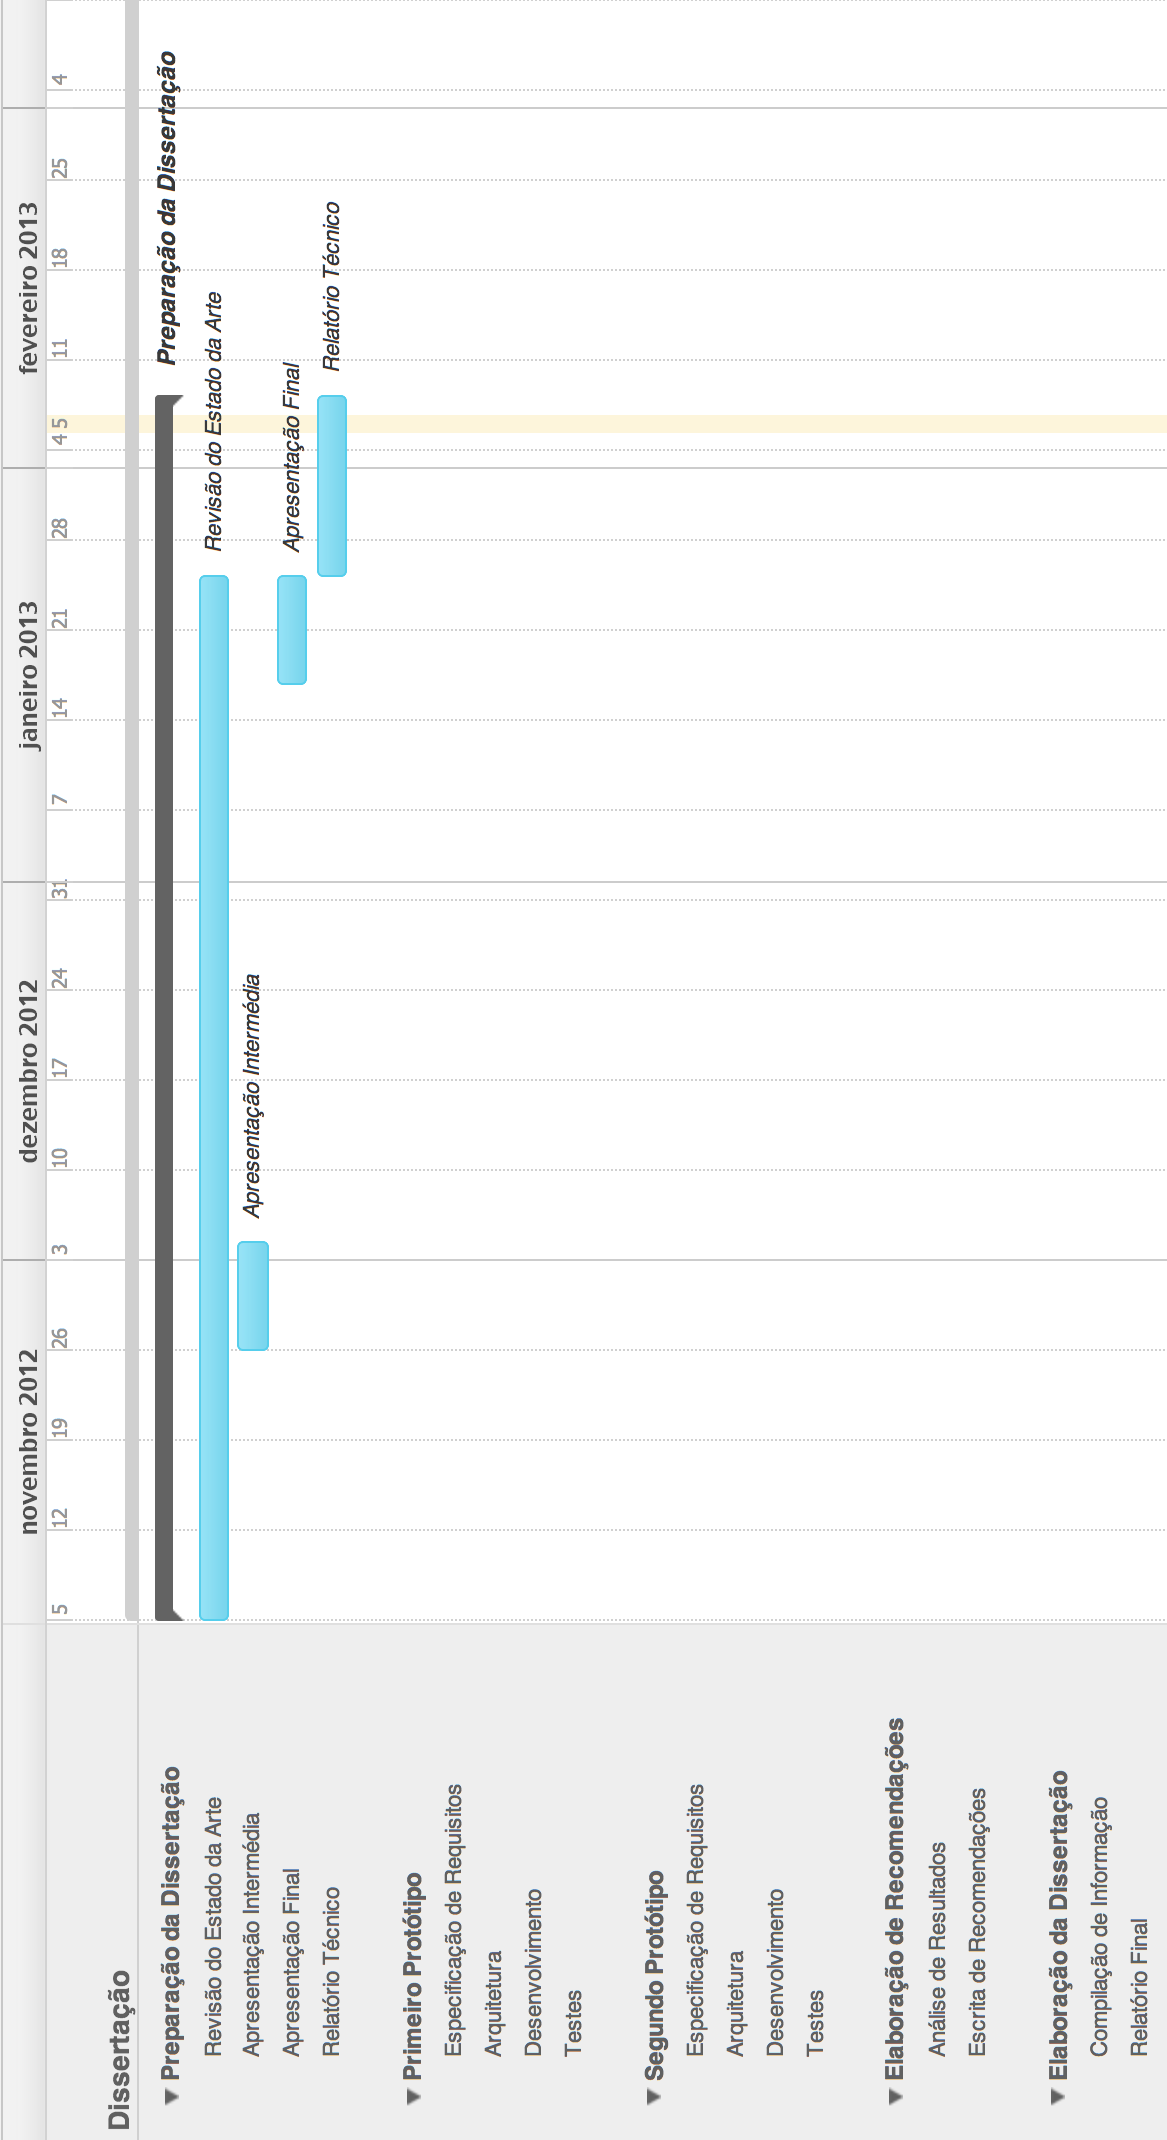
\includegraphics[height=23cm]{gantt_part1}
    \caption{Planeamento da primeira fase da dissertação}
    \label{fig:gantt1}
  \end{center}
\end{figure}

\begin{figure}[t]
  \begin{center}
    \leavevmode
    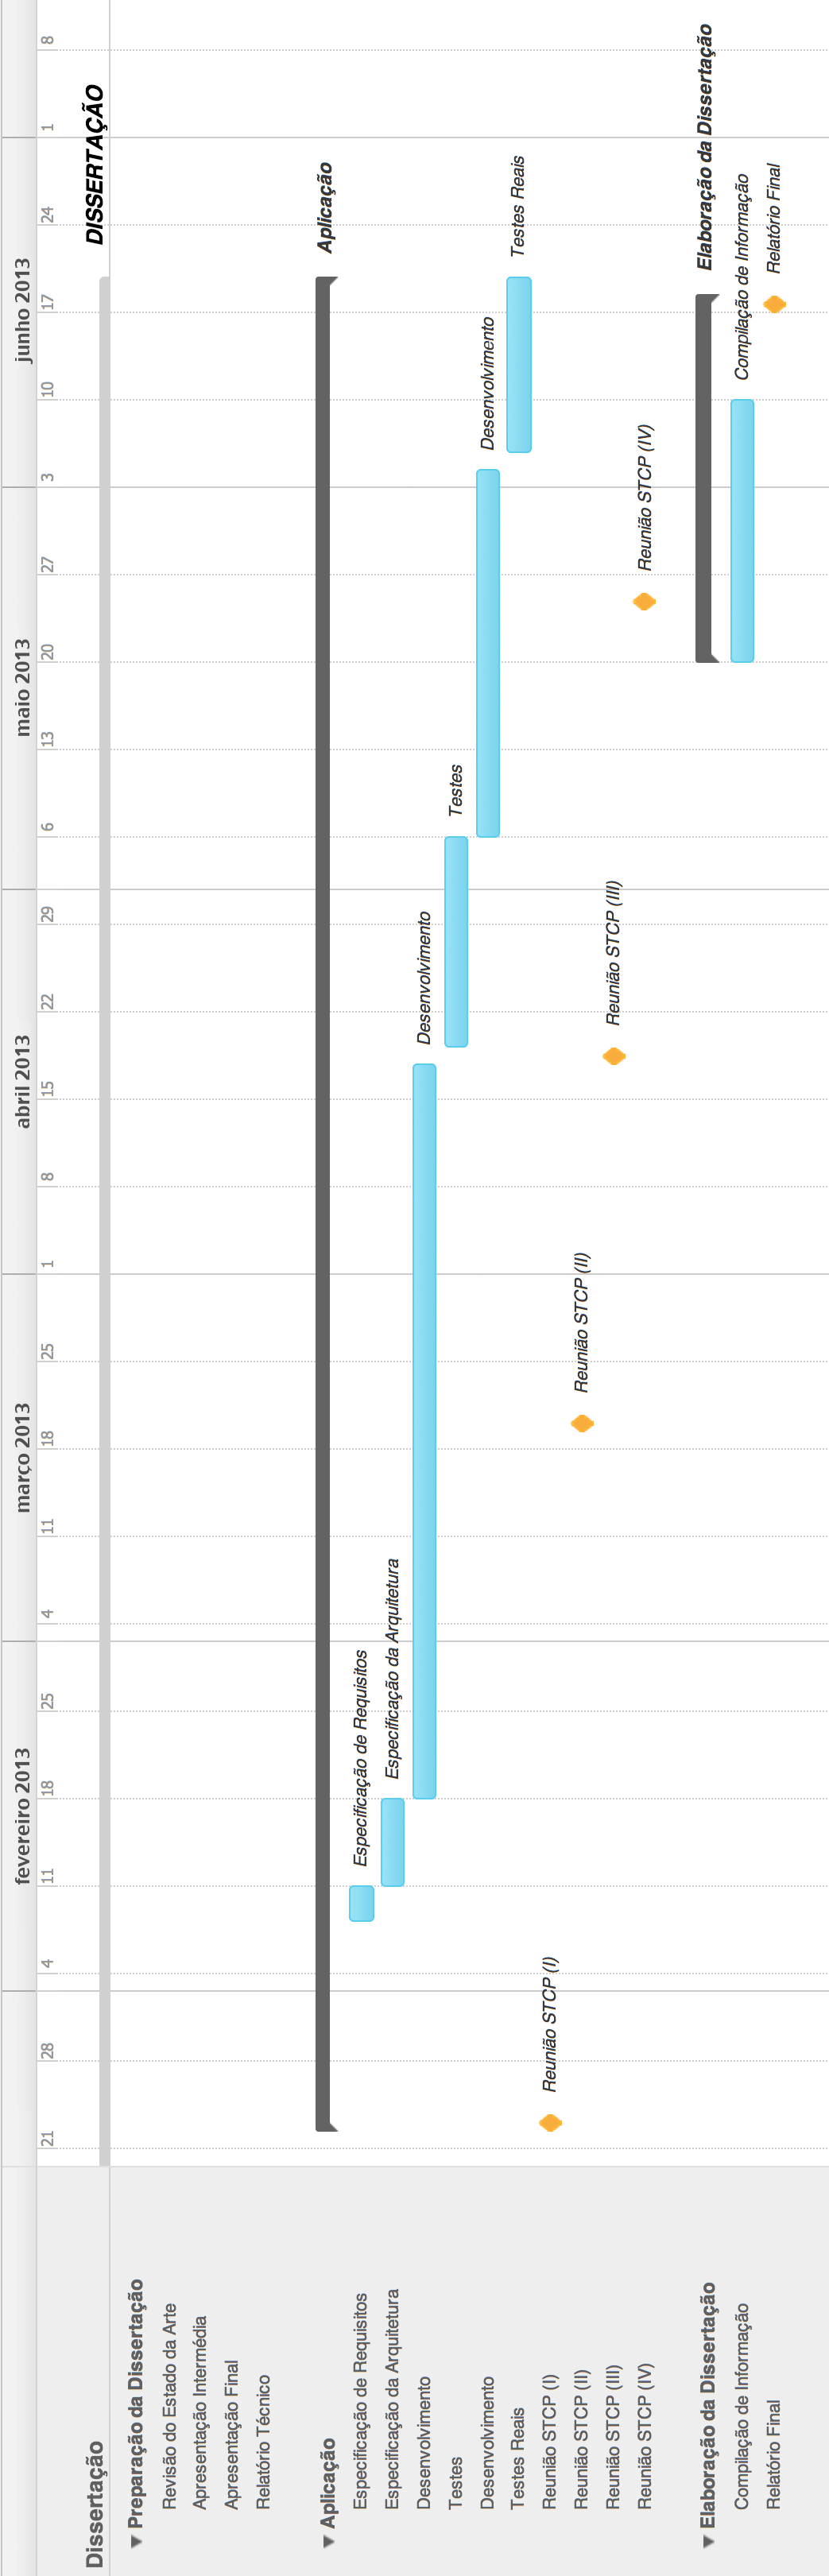
\includegraphics[height=23cm]{gantt_part2}
    \caption{Planeamento da segunda fase da dissertação}
    \label{fig:gantt2}
  \end{center}
\end{figure}

\section{Trabalho Futuro}

Esta dissertação pode ser considerada como uma primeira abordagem à criação de uma solução para a bilhética móvel aplicada aos transportes públicos de passageiros, havendo, portanto, ainda um longo caminho a percorrer até se atingir todo o potencial deste conceito. Como tal, há uma série de funcionalidades e características que podem ser objeto de mudança no futuro.
\\Durante o desenvolvimento da aplicação, havia a perfeita noção de que o tempo era limitado e portanto havia a necessidade de implementar apenas as funcionalidades essenciais para o bom funcionamento da aplicação, mas todas as novas ideias foram sendo registadas, para posterior análise e implementação. Caso contrário, não seria possível terminar o desenvolvimento da aplicação e dar início à fase de testes, pois a cada passo novas ideias de como melhorar a aplicação iam surgindo.

~\\De seguida, são apresentadas várias partes do projeto que necessitam ainda de ser exploradas e melhoradas, dado que o sucesso da aplicação poderá passar pela implementação dessas alterações.

\subsection{Estrutura de Dados}

Tendo em conta a necessidade de comunicação constante com o servidor, é necessário avaliar qual a informação estritamente necessária em cada momento e cingir a aplicação à utilização da mesma, permitindo reduzir o tempo de operação e o tráfego de dados, apesar de este já ser residual.
\\Para além disso, é necessário reestruturar a base de dados local, de modo a permitir implementar algumas funcionalidades previstas, nomeadamente a seleção de paragens favoritas ou histórico de paragens.
\\É necessário também criar uma estrutura de comunicação de imagens, tanto para a fotografia do utilizador, como para os fundos do Menu Revisor, passando esta informação a estar centralizada no servidor.

\subsection{Segurança}

Apesar de, na sua estrutura, a aplicação já estar preparada para utilizar comunicação encriptada através de conjuntos de chaves públicas e privadas, é necessário implementar essa camada de segurança, bem como prever e eliminar casos de replicação ou adulteração de pedidos. Tendo em conta que a aplicação envolve transações monetárias, é fundamental que esta se apresente como uma solução segura.
\\A nível de segurança do utilizador, é necessário criar mecanismos de recuperação de palavra-passe e dupla verificação dos dados sensíveis.

\subsection{Carregamento de Conta}

Neste momento, a aplicação apenas permite efetuar compras de títulos com o saldo disponível na conta do utilizador. O próximo passo será o carregamento da conta, havendo várias possibilidades de o fazer. É necessário estudar a viabilidade das várias opções, bem como os seus custos. O ideal será, para o utilizador, não ter custos adicionais na utilização da aplicação, caso contrário haverá alguma relutância em deixar o sistema de bilhética atual. Entre as opções possíveis, está a possibilidade de utilizar o saldo do próprio telemóvel, sendo necessário estudar o caso junto das operadoras móveis; o carregamento através do sistema MB Phone ou PayPal, utilizando as ferramentas já existentes; a associação a uma conta bancária, sendo o débito feito diretamente, tal como acontece nas portagens Via Verde.
\\Um dos requisitos fundamentais é que a disponibilidade de saldo tem de ser imediata após o carregamento, porque é inviável para um utilizador que precisa de efetuar uma viagem e correspondente carregamento, ter de esperar mais do que alguns segundos para poder proceder à compra do título que necessita.

\subsection{Validação}

Os testes mostraram que o processo de validação é o que necessita de mais revisão e simplificação. É necessário estudar eventuais alternativas à necessidade de escolha de paragem e linha de entrada, bem como tornar este processo mais rápido e com menos margem de erro.
\\O sistema de localização mostrou ser pouco eficiente, devido às limitações temporais e também à densidade urbana que se apresenta em algumas das localizações das paragens. Deste modo, é necessário criar alternativas que permitam, de forma inequívoca, assinalar qual a paragem e linha de entrada.
\\Para além do problema da localização, surge outro problema que é o facto de haver desvios nos trajetos dos veículos, levando à criação de paragens temporárias, bem como a mudança de local de algumas paragens. Se o sistema não estiver preparado para essas alterações, não será possível validar corretamente.

\subsection{Outros}

Sendo objetivo final da aplicação, a integração com a aplicação MOVE-ME, uma das funcionalidades pensadas é a possibilidade de escolher determinado percurso (já possível na aplicação MOVE-ME) e proceder à compra do título mais adequado a esse trajeto. Esta funcionalidade será bastante útil para viagens que fujam à rotina diária e também para os turistas, que muitas vezes encontram dificuldades na hora da compra de títulos.
\\A nível do utilizador, está planeado fornecer futuramente informação estatística, aconselhando-o a trocar de tipo de títulos conforme a necessidade, ou seja, um utilizador que efetue poucas viagens e possua uma assinatura mensal, será aconselhado a optar por títulos de viagem ocasionais, e vice-versa.
\\A possibilidade de envio ou troca de títulos entre utilizadores, permite que em caso de necessidade seja possível emprestar ou dar títulos ocasionais a outra pessoa, permitindo dessa forma evitar gastos desnecessários e ao mesmo tempo utilizar vários títulos que não poderiam ser utilizados em simultâneo. Exemplificando, hoje em dia se a pessoa A tiver 2 títulos de viagem no seu cartão e a pessoa B não tiver nenhum e quiserem viajar juntas, a pessoa A validará um dos títulos que possui (ficando o outro armazenado no cartão) e a pessoa B terá obrigatoriamente de comprar um título de viagem.
\\Do ponto de vista dos operadores, a possibilidade de aceder a dados massivos acerca dos hábitos dos seus passageiros, permite que planeiem melhor as suas rotas, definam tarifários adequados e forneçam um melhor serviço, aumentando assim a visibilidade da marca e a satisfação global dos passageiros.
\\Tudo isto são funcionalidades que não estão ainda disponíveis no sistema atual e, como tal, trariam uma grande mais-valia ao projeto.

~\\Para além de todas as funcionalidades aqui descritas, serão tidas em conta as várias sugestões apresentadas pelos utilizadores durante a fase de testes, que podem ser consultadas na Secção~\ref{sec:sugestoes}.

\section{Resumo}

Há ainda muito trabalho a desenvolver, e os parceiros estão interessados em dar continuidade ao projeto por considerarem ser um conceito inovador e prático. O facto de cada vez mais utilizadores dos transportes públicos serem possuidores de dispositivos móveis, consumindo informação constantemente, abre as portas à bilhética móvel, não havendo quaisquer entraves por parte do utilizador, que se mostra bastante satisfeito com a comodidade e simplicidade presentes no conceito.
\\Uma outra vantagem deste sistema face a outros na mesma área, é a remoção de quaisquer intervenientes físicos durante todo o processo de utilização. Todas as operações são realizadas através dos dispositivos móveis. No entanto, este sistema tira proveito de um modelo de transportes sem barreiras, como é o caso da Área Metropolitana do Porto, não sendo possível implementá-lo em sistemas fechados sem as devidas modificações que permitissem comunicar com os sistemas de barreiras.

~\\Numa conclusão geral, o conceito está aprovado, é viável e é agora necessário torná-lo robusto e simples de modo a que possa ser utilizado por todos os operadores de transportes públicos da Área Metropolitana do Porto, trazendo-lhes informações adicionais sobre os seus passageiros e também fornecendo aos utilizadores uma solução prática, cómoda e eficaz para as suas deslocações.